\documentclass[../notes.tex]{subfiles}

\pagestyle{main}
\renewcommand{\chaptermark}[1]{\markboth{\chaptername\ \thechapter\ (#1)}{}}
\setcounter{chapter}{6}

\begin{document}




\chapter{Bonding in Coordination Complexes}
\section[Coordination Complexes: \texorpdfstring{$\pi$}{TEXT} Bonding and all-\texorpdfstring{$\sigma$}{TEXT} Distortions]{Coordination Complexes: \texorpdfstring{$\bm{\pi}$}{TEXT} Bonding and all-\texorpdfstring{$\bm{\sigma}$}{TEXT} Distortions}
\begin{itemize}
    \item \marginnote{11/7:}Video lecture Wed and Fri; watch by Mon and have questions.
    \item Last time: MO diagram for an \ce{ML6} coordination complex whose ligands only engage in $\sigma$ interactions.
    \item Today: The case where the ligands also have $\pi$ orbitals.
    \item As per usual, we follow the procedure from Lecture 6.1.
    \begin{enumerate}
        \item Point group: $O_h$.
        \item Assigning coordinate axes is a bit more complicated here, but the following will work.
        \begin{figure}[h!]
            \centering
            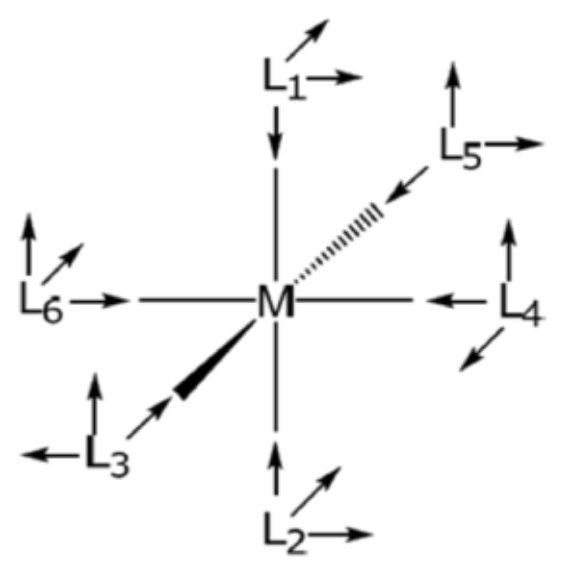
\includegraphics[width=0.2\linewidth]{../ExtFiles/piOrientationsML6.png}
            \caption{\ce{ML6} $\pi$ $xyz$ coordinates.}
            \label{fig:xyzML6pi}
        \end{figure}
        \begin{itemize}
            \item We have two orthogonal $p\pi$ bonds.
            \item The arrows indicate the directional phase of the $p$ orbitals.
        \end{itemize}
        \item Let's create a representation for the 12 $p$ orbitals capable of $\pi$ bonding.
        \begin{table}[h!]
            \centering
            \small
            \renewcommand{\arraystretch}{1.2}
            \begin{tabular}{c|cccccccccc}
                $O_h$ & $E$ & $8C_3$ & $6C_2$ & $6C_4$ & $3C_2$ & $i$ & $6S_4$ & $8S_6$ & $3\sigma_h$ & $6\sigma_d$\\
                \hline
                $\Gamma_{12\pi}$ & 12 & 0 & 0 & 0 & $-4$ & 0 & 0 & 0 & 0 & 0\\
            \end{tabular}
            \caption{Representation for the $p\pi$ ligand orbitals of \ce{ML6}.}
            \label{tab:ML6pRR}
        \end{table}
        \item Reducing, we get
        \begin{equation*}
            \Gamma_{12\pi} = T_{1g}+T_{1u}+T_{2g}+T_{2u}
        \end{equation*}
        \item From Table \ref{tab:charTableOh}, the atomic orbitals of the metal transform as
        \begin{align*}
            s &\sim a_{1g}&
            p_x,p_y,p_z &\sim t_{1u}&
            d_{z^2},d_{x^2-y^2} &\sim e_g&
            d_{xz},d_{yz},d_{xy} &\sim t_{2g}
        \end{align*}
        \begin{itemize}
            \item Thus, the metal $p$ and $d_{xz},d_{yz},d_{xy}$ orbitals interact with the ligand $\pi$ SALCS.
        \end{itemize}
        \pagebreak
        \item Once again, we can "guess" the SALCs based on experience.
        \begin{figure}[H]
            \centering
            \begin{subfigure}[b]{0.24\linewidth}
                \centering
                \begin{tikzpicture}
                    \footnotesize
                    \draw
                        (0,0) coordinate (M) -- ++(90:4em)   coordinate (L1)
                        (0,0)                -- ++(-160:4em) coordinate (L2)
                        (0,0)                -- ++(-20:4em)  coordinate (L3)
                        (0,0)                -- ++(20:4em)   coordinate (L4)
                        (0,0)                -- ++(160:4em)  coordinate (L5)
                        (0,0)                -- ++(-90:4em)  coordinate (L6)
                    ;
        
                    \filldraw [semithick,fill=white] (M)
                        to[out=0,in=0,out looseness=0.5] ++(0,0.5)
                        to[out=180,in=180,in looseness=0.5] cycle
                    ;
                    \filldraw [semithick,fill=grz] (M)
                        to[out=0,in=0,out looseness=0.5] ++(0,-0.5)
                        to[out=180,in=180,in looseness=0.5] cycle
                    ;
                    \foreach \n in {L2,L3,L4,L5} {
                        \filldraw [semithick,fill=white] (\n)
                            to[out=0,in=0,out looseness=0.5] ++(0,0.3)
                            to[out=180,in=180,in looseness=0.5] cycle
                        ;
                        \filldraw [semithick,fill=grz] (\n)
                            to[out=0,in=0,out looseness=0.5] ++(0,-0.3)
                            to[out=180,in=180,in looseness=0.5] cycle
                        ;
                    }
                \end{tikzpicture}
                \caption{$t_{1u}$ bonding.}
                \label{fig:SALCML6pia}
            \end{subfigure}
            \begin{subfigure}[b]{0.24\linewidth}
                \centering
                \begin{tikzpicture}
                    \footnotesize
                    \draw
                        (0,0) coordinate (M) -- ++(90:4em)   coordinate (L1)
                        (0,0)                -- ++(-160:4em) coordinate (L2)
                        (0,0)                -- ++(-20:4em)  coordinate (L3)
                        (0,0)                -- ++(20:4em)   coordinate (L4)
                        (0,0)                -- ++(160:4em)  coordinate (L5)
                        (0,0)                -- ++(-90:4em)  coordinate (L6)
                    ;
        
                    \filldraw [semithick,fill=white,rotate=0,yscale=0.6] (M)
                        to[out=0,in=0,out looseness=0.5,in looseness=1.5] ++(0,0.65)
                        to[out=180,in=180,out looseness=1.5,in looseness=0.5] cycle
                    ;
                    \filldraw [semithick,fill=grz,rotate=-90] (M)
                        to[out=0,in=0,out looseness=0.5,in looseness=1.5] ++(0,0.65)
                        to[out=180,in=180,out looseness=1.5,in looseness=0.5] cycle
                    ;
                    \filldraw [semithick,fill=grz,rotate=90] (M)
                        to[out=0,in=0,out looseness=0.5,in looseness=1.5] ++(0,0.65)
                        to[out=180,in=180,out looseness=1.5,in looseness=0.5] cycle
                    ;
                    \filldraw [semithick,fill=white,rotate=180,yscale=0.6] (M)
                        to[out=0,in=0,out looseness=0.5,in looseness=1.5] ++(0,0.65)
                        to[out=180,in=180,out looseness=1.5,in looseness=0.5] cycle
                    ;
        
                    \foreach \n/\a in {L2/-110,L3/110,L4/70,L5/-70} {
                        \filldraw [semithick,fill=white,rotate=\a] (\n)
                            to[out=0,in=0,out looseness=0.5] ++(0,0.3)
                            to[out=180,in=180,in looseness=0.5] cycle
                        ;
                        \filldraw [semithick,fill=grz,rotate=\a] (\n)
                            to[out=0,in=0,out looseness=0.5] ++(0,-0.3)
                            to[out=180,in=180,in looseness=0.5] cycle
                        ;
                    }
                \end{tikzpicture}
                \caption{$t_{2g}$ bonding.}
                \label{fig:SALCML6pib}
            \end{subfigure}
            \begin{subfigure}[b]{0.24\linewidth}
                \centering
                \begin{tikzpicture}
                    \footnotesize
                    \draw
                        (0,0) coordinate (M) -- ++(90:4em)   coordinate (L1)
                        (0,0)                -- ++(-160:4em) coordinate (L2)
                        (0,0)                -- ++(-20:4em)  coordinate (L3)
                        (0,0)                -- ++(20:4em)   coordinate (L4)
                        (0,0)                -- ++(160:4em)  coordinate (L5)
                        (0,0)                -- ++(-90:4em)  coordinate (L6)
                    ;
        
                    \foreach \n/\a in {L2/-110,L3/-70,L4/70,L5/110} {
                        \filldraw [semithick,fill=white,rotate=\a] (\n)
                            to[out=0,in=0,out looseness=0.5] ++(0,0.3)
                            to[out=180,in=180,in looseness=0.5] cycle
                        ;
                        \filldraw [semithick,fill=grz,rotate=\a] (\n)
                            to[out=0,in=0,out looseness=0.5] ++(0,-0.3)
                            to[out=180,in=180,in looseness=0.5] cycle
                        ;
                    }
                \end{tikzpicture}
                \caption{$t_{1g}$ nonbonding.}
                \label{fig:SALCML6pic}
            \end{subfigure}
            \begin{subfigure}[b]{0.24\linewidth}
                \centering
                \begin{tikzpicture}
                    \footnotesize
                    \draw
                        (0,0) coordinate (M) -- ++(90:4em)   coordinate (L1)
                        (0,0)                -- ++(-160:4em) coordinate (L2)
                        (0,0)                -- ++(-20:4em)  coordinate (L3)
                        (0,0)                -- ++(20:4em)   coordinate (L4)
                        (0,0)                -- ++(160:4em)  coordinate (L5)
                        (0,0)                -- ++(-90:4em)  coordinate (L6)
                    ;
        
                    \foreach \n/\a in {L2/0,L3/180,L4/0,L5/180} {
                        \filldraw [semithick,fill=white,rotate=\a] (\n)
                            to[out=0,in=0,out looseness=0.5] ++(0,0.3)
                            to[out=180,in=180,in looseness=0.5] cycle
                        ;
                        \filldraw [semithick,fill=grz,rotate=\a] (\n)
                            to[out=0,in=0,out looseness=0.5] ++(0,-0.3)
                            to[out=180,in=180,in looseness=0.5] cycle
                        ;
                    }
                \end{tikzpicture}
                \caption{$t_{2u}$ nonbonding.}
                \label{fig:SALCML6pid}
            \end{subfigure}
            \caption{\ce{ML6} $\pi$ SALCs.}
            \label{fig:SALCML6pi}
        \end{figure}
        \begin{itemize}
            \item In addition to these, there are two more (oriented along the other orthogonal coordinate axes) for each IRR.
        \end{itemize}
        \item We can now make sense of the MO diagram.
        \begin{figure}[h!]
            \centering
            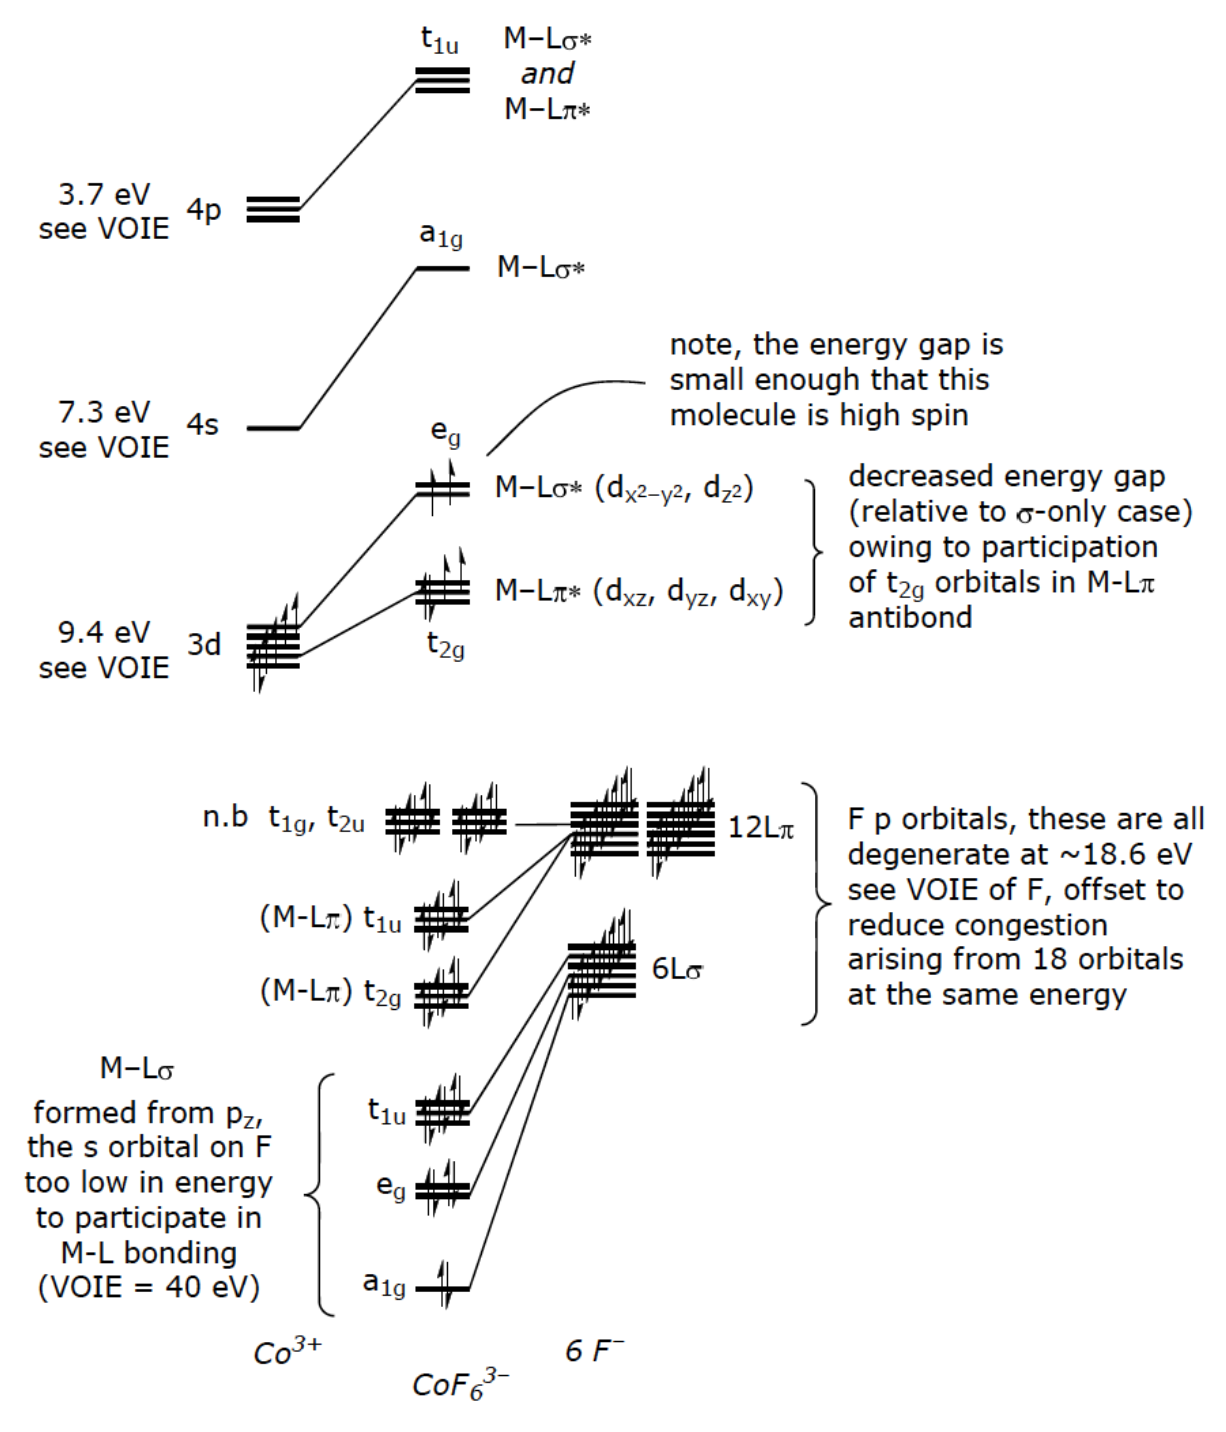
\includegraphics[width=0.6\linewidth]{../ExtFiles/MOsML6pi.png}
            \caption{\ce{ML6} $\pi$ MO diagram.}
            \label{fig:MOsML6pi}
        \end{figure}
        \begin{itemize}
            \item Wuttig compares this MO diagram to the all-$\sigma$ case (Figure \ref{fig:MOsML6}).
            \begin{itemize}
                \item The \ce{M}-\ce{L\sigma} and \ce{M}-\ce{L\sigma^*} distortions stay the same; we now just have \emph{additional} \ce{M}-\ce{L\pi} and \ce{M}-\ce{L\pi^*} distortions to consider.
                \item $\pi$-donating ligands, such as the fluoride ligands causing the interactions in Figure \ref{fig:MOsML6pi}, \emph{raise} the $t_{2g}$ set in energy; they contribute \emph{antibonding} interactions.
                \item Note that the \ce{L\pi} orbitals sit above the \ce{L\sigma} orbitals.
            \end{itemize}
            \item Wuttig probably expects us to be familiar with the \ce{M}-\ce{L\pi^*} notation.
        \end{itemize}
    \end{enumerate}
    \item It seems that now we're done. But wait: We have made an assumption that is not necessarily justified in every case.
    \begin{itemize}
        \item We have treated the ligand as a point particle with atomic orbitals that mirror the metal center (i.e., your typical $s$, $p$, etc. orbitals).
        \item This is justified in the case of fluoride (as in Figure \ref{fig:MOsML6pi}). But what about a ligand such as carbon monoxide? \ce{CO} certainly has molecular orbitals more complicated than the atomic orbitals of either carbon or oxygen alone, so is it still valid to treat it as a point particle with "atomic" orbitals?
        \item In fact, it is not, and we will now see how to treat that case.
    \end{itemize}
    \item As with fluoride, the frontier orbitals of \ce{CO} will be the ones that interact with the metal center.
    \item To draw SALCs of the interactions of these MOs with the metal center, we need to know what \emph{they} look like first. Fortunately, we have encountered the SALCs for heteronuclear diatomics before, and we can simply use these as our basis set to draw the overall SALCs.
    \begin{figure}[h!]
        \centering
        \begin{subfigure}[b]{0.24\linewidth}
            \centering
            \begin{tikzpicture}
                \footnotesize
                \draw
                    (0,0) coordinate (M) -- ++(90:4em)   coordinate (L1)
                    (0,0)                -- ++(-160:4em) coordinate (L2)
                    (0,0)                -- ++(-20:4em)  coordinate (L3)
                    (0,0)                -- ++(20:4em)   coordinate (L4)
                    (0,0)                -- ++(160:4em)  coordinate (L5)
                    (0,0)                -- ++(-90:4em)  coordinate (L6)
                ;
    
                \filldraw [semithick,fill=white] (M)
                    to[out=0,in=0,out looseness=0.5] ++(0,0.5)
                    to[out=180,in=180,in looseness=0.5] cycle
                ;
                \filldraw [semithick,fill=grz] (M)
                    to[out=0,in=0,out looseness=0.5] ++(0,-0.5)
                    to[out=180,in=180,in looseness=0.5] cycle
                ;
                \foreach \n in {L2,L3,L4,L5} {
                    \filldraw [semithick,fill=white] ($(M)!0.8!(\n)$)
                        to[out=0,in=0,out looseness=0.5] ++(0,0.3)
                        to[out=180,in=180,in looseness=0.5] cycle
                    ;
                    \filldraw [semithick,fill=grz] ($(M)!0.8!(\n)$)
                        to[out=0,in=0,out looseness=0.5] ++(0,-0.3)
                        to[out=180,in=180,in looseness=0.5] cycle
                    ;
                    \filldraw [semithick,fill=white] (\n)
                        to[out=0,in=0,out looseness=0.5] ++(0,-0.3)
                        to[out=180,in=180,in looseness=0.5] cycle
                    ;
                    \filldraw [semithick,fill=grz] (\n)
                        to[out=0,in=0,out looseness=0.5] ++(0,0.3)
                        to[out=180,in=180,in looseness=0.5] cycle
                    ;
                }
            \end{tikzpicture}
            \caption{$t_{1u}$ bonding.}
            \label{fig:SALCMCO6a}
        \end{subfigure}
        \begin{subfigure}[b]{0.24\linewidth}
            \centering
            \begin{tikzpicture}
                \footnotesize
                \draw
                    (0,0) coordinate (M) -- ++(90:4em)   coordinate (L1)
                    (0,0)                -- ++(-160:4em) coordinate (L2)
                    (0,0)                -- ++(-20:4em)  coordinate (L3)
                    (0,0)                -- ++(20:4em)   coordinate (L4)
                    (0,0)                -- ++(160:4em)  coordinate (L5)
                    (0,0)                -- ++(-90:4em)  coordinate (L6)
                ;
    
                \filldraw [semithick,fill=white,rotate=0,yscale=0.6] (M)
                    to[out=0,in=0,out looseness=0.5,in looseness=1.5] ++(0,0.65)
                    to[out=180,in=180,out looseness=1.5,in looseness=0.5] cycle
                ;
                \filldraw [semithick,fill=grz,rotate=-90] (M)
                    to[out=0,in=0,out looseness=0.5,in looseness=1.5] ++(0,0.65)
                    to[out=180,in=180,out looseness=1.5,in looseness=0.5] cycle
                ;
                \filldraw [semithick,fill=grz,rotate=90] (M)
                    to[out=0,in=0,out looseness=0.5,in looseness=1.5] ++(0,0.65)
                    to[out=180,in=180,out looseness=1.5,in looseness=0.5] cycle
                ;
                \filldraw [semithick,fill=white,rotate=180,yscale=0.6] (M)
                    to[out=0,in=0,out looseness=0.5,in looseness=1.5] ++(0,0.65)
                    to[out=180,in=180,out looseness=1.5,in looseness=0.5] cycle
                ;
    
                \foreach \n/\a in {L2/-110,L3/110,L4/70,L5/-70} {
                    \filldraw [semithick,fill=white,rotate=\a] ($(M)!0.8!(\n)$)
                        to[out=0,in=0,out looseness=0.5] ++(0,0.3)
                        to[out=180,in=180,in looseness=0.5] cycle
                    ;
                    \filldraw [semithick,fill=grz,rotate=\a] ($(M)!0.8!(\n)$)
                        to[out=0,in=0,out looseness=0.5] ++(0,-0.3)
                        to[out=180,in=180,in looseness=0.5] cycle
                    ;
                    \filldraw [semithick,fill=white,rotate=\a] (\n)
                        to[out=0,in=0,out looseness=0.5] ++(0,-0.3)
                        to[out=180,in=180,in looseness=0.5] cycle
                    ;
                    \filldraw [semithick,fill=grz,rotate=\a] (\n)
                        to[out=0,in=0,out looseness=0.5] ++(0,0.3)
                        to[out=180,in=180,in looseness=0.5] cycle
                    ;
                }
            \end{tikzpicture}
            \caption{$t_{2g}$ bonding.}
            \label{fig:SALCMCO6b}
        \end{subfigure}
        \caption{\ce{M(CO)6} $\pi$-bonding SALCs.}
        \label{fig:SALCMCO6}
    \end{figure}
    \begin{itemize}
        \item Wuttig draws the Figure \ref{fig:SALCMCO6a} interactions in-plane, too, though??
        \item Wuttig also doesn't draw the nonbonding ones, but they still exist??
        \item To reiterate, the $\pi^*$ orbitals of \ce{CO} will participate in $t_{1u}$ and $t_{2g}$ bonding interactions, and $t_{1g}$ and $t_{2u}$ nonbonding interactions just like the $p$ orbitals of \ce{F}; it is \emph{strictly} and \emph{solely} the basis set that we're changing.
    \end{itemize}
    \item An additional complication arises from the fact that the frontier orbitals of \ce{CO} are fundamentally different than those of \ce{F}.
    \begin{itemize}
        \item In particular, the frontier orbitals of \ce{F} are filled $\pi$-donating atomic orbitals, while \ce{CO} has a filled $\sigma$-donating frontier orbital (HOMO) and an unfilled $\pi^*$-accepting frontier orbital (LUMO).
        \item Thus, we need to consider the new \emph{energetics} of these orbitals as well.
        \item For a $\pi$-donating ligand such as monoatomic fluoride, the $\sigma$ and $\pi$ orbitals are degenerate.
        \begin{itemize}
            \item This is because all 18 ligand orbitals come from the $2p$ \emph{atomic} orbitals of fluorine.
        \end{itemize}
        \item However\dots
    \end{itemize}
    \item Are the $\sigma$ and $\pi$ orbitals of the $\pi$-accepting ligands degenerate in energy?
    \begin{itemize}
        \item They are not.
        \item This is because we are considering the interactions of nondegenerate ligand \emph{molecular} orbitals with the metal center.
        \item Evidence: We can inspect the photoelectron spectrum of our ligand (e.g., for \ce{CO}, we observe distinct peaks corresponding to its $\sigma$-donating and $\pi^*$-accepting orbitals).
        \item Note that ligands such as \ce{CO} still have filled $\pi$ MOs; it's just that these lie so low in energy that they don't interact with the metal center.
    \end{itemize}
    \item The consequence of this is that the $\pi$ ligand orbitals of a $\pi$-accepting ligand lie significantly higher in energy.
    \begin{itemize}
        \item In fact, they lie higher in energy than a metal's $d$ orbitals, meaning that the metal $t_{2g}$ set is now \ce{M}-\ce{L\pi} \emph{bonding} instead of \emph{antibonding} and hence lower in energy, leading to a greater $d$ orbital splitting.
    \end{itemize}
    \item All of this can be summarized by the MO diagram for a \ce{ML6} complex with $\pi$-accepting ligands.
    \begin{figure}[h!]
        \centering
        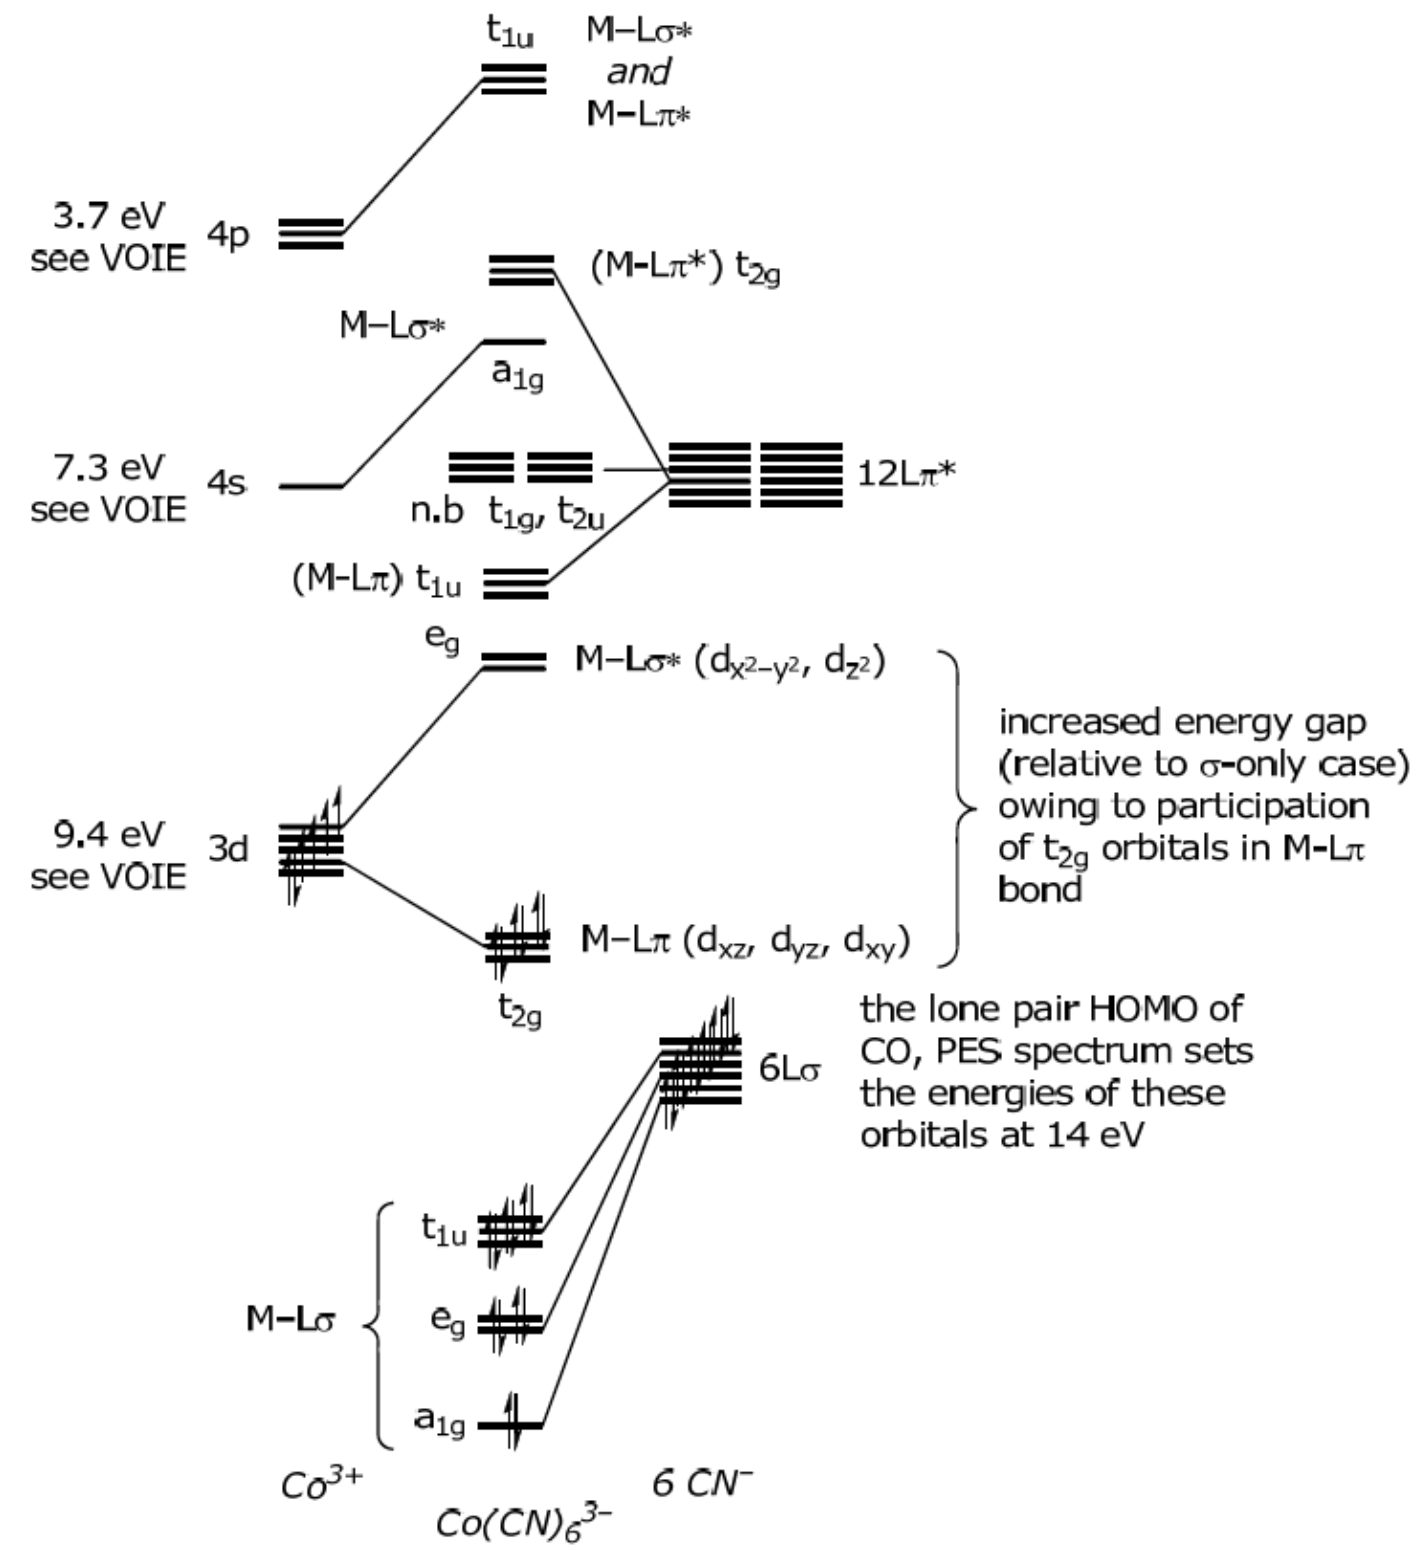
\includegraphics[width=0.6\linewidth]{../ExtFiles/MOsML6piAcc.png}
        \caption{\ce{ML6} $\pi$-accepting MO diagram.}
        \label{fig:MOsML6piAcc}
    \end{figure}
    \item Distortions from $\sigma$ interactions.
    \item Consider a \ce{ML6} complex with $\sigma$-only interactions, as discussed last class.
    \begin{itemize}
        \item Goal: Predict Jahn-Teller distortions from first principles.
        \item Two possible distortions: A tetragonal compression or a Jahn-Teller elongation.
        \begin{itemize}
            \item See Figure VI.10 of \textcite{bib:CHEM20100Notes}.
            \item Are both of these distortions not "Jahn-Teller" effects??
        \end{itemize}
        \item Either distortion changes the point group from $O_h$ to $D_{4h}$.
    \end{itemize}
    \item We now seek to build an MO diagram for the $t_{2g}$ and $e_g$ set of each distortion.
    \begin{table}[h!]
        \centering
        \small
        \renewcommand{\arraystretch}{1.2}
        \begin{tabular}{c|c|c}
             & $O_h$ & $D_{4h}$\\
            \hline
            $d_{x^2-y^2}$ & $e_g$ & $b_{1g}$\\
            $d_{z^2}$ & $e_g$ & $a_{1g}$\\
            $d_{xy}$ & $t_{2g}$ & $b_{2g}$\\
            $d_{yz}$ & $t_{2g}$ & $e_g$\\
            $d_{xz}$ & $t_{2g}$ & $e_g$\\
        \end{tabular}
        \caption{$d$-orbital symmetries in $O_h$ vs. $D_{4h}$.}
        \label{tab:dOrbOhD4h}
    \end{table}
    \begin{itemize}
        \item To begin, we determine the symmetries are the $d$ orbitals in the two point groups (see Table \ref{tab:dOrbOhD4h}).
        \item Since the $t_{2g}$ set is nonbonding in a $\sigma$-only complex, their energy doesn't change much, so the distorted $t_{2g}$ set is basically still degenerate. However, we do have to draw the $b_{2g}$ MO slightly higher (or lower, but we choose higher) since it has a different symmetry.
        \item The $e_g$ orbitals definitively split, going in different directions as the axial ligands compress or expand. In particular, compressing the axial ligands drives $d_{z^2}$ up (and $d_{x^2-y^2}$ down), and vice versa for expanding the axial ligands.
        \item Note that the original $e_g$ set is \ce{M}-\ce{L\sigma^*}, which is why compression drives up energy (more mixing between regions of opposite phases is not energetically favorable).
    \end{itemize}
\end{itemize}



\section{Descent in Symmetry}
\begin{itemize}
    \item \marginnote{11/9:}Goal: Consequences of distortion and descent in symmetry on the MOs of coordination complexes.
    \item \textbf{Homoleptic}: A coordination complex, the ligands of which are all identical.
    \item \textbf{Heteroleptic}: A coordination complex containing at least two distinct ligands.
    \item Most interesting chemistry occurs for heteroleptics, so we should consider their MOs, too.
    \item But how do we construct such molecular orbitals? Use a Descent in Symmetry Analysis.
    \begin{itemize}
        \item Similar to the Jahn-Teller distortion and tetragonal compression discussed in Lecture 16, but now we're taking this a step further by fully removing ligands. We then investigate the effects of this on orbital energetics.
    \end{itemize}
    \item How do the symmetries of the $d$ orbitals compare from \ce{Co(CN)6} to the hypothetical "chopped off \ce{Co(CN)5} complex," i.e., $C_{4v}$ fragment?
    \begin{itemize}
        \item We rip a cyano group off of the axial position and will substitute a bromo group later.
        \item Changing from $O_h$ to $C_{4v}$ involves a change in the symmetries of the orbitals, as follows.
        \begin{table}[h!]
            \centering
            \small
            \renewcommand{\arraystretch}{1.2}
            \begin{tabular}{c|c|c}
                 & $O_h$ & $C_{4v}$\\
                \hline
                $d_{x^2-y^2}$ & $e_g$ & $b_1$\\
                $d_{z^2}$ & $e_g$ & $a_1$\\
                $d_{xz}$ & $t_{2g}$ & $e$\\
                $d_{yz}$ & $t_{2g}$ & $e$\\
                $d_{xy}$ & $t_{2g}$ & $b_2$\\
            \end{tabular}
            \caption{$d$-orbital symmetries in $O_h$ vs. $C_{4v}$.}
            \label{tab:dOrbOhC4v}
        \end{table}
        \item Taking a $\pi$-acceptor off of the $z$-axis won't affect $d_{x^2-y^2}$; we just change the label from $e_g\mapsto b_1$.
        \item Since $d_{z^2}$ now has a less productive $\sigma$-bonding interaction, the \ce{M}-\ce{L\sigma^*} $d_{z^2}$ orbital decreases in energy (and changes to $a_1$).
        \item As with $d_{x^2-y^2}$, $d_{xy}$ doesn't change except in symmetry.
        \item Analogously to $d_{z^2}$, $d_{xz}$ and $d_{yz}$ now increase in energy because we lose the stabilizing effect of the $\pi^*$ ligand acceptance.
    \end{itemize}
    \item Now what happens when we add \ce{Br-} back in?
    \begin{itemize}
        \item \ce{Br-} is a $\pi$-donor!
        \item Quantitatively, we need to find the symmetry of the \ce{Br-} atomic orbitals and mix them with the MOs of the fragment.
        \item Since $p_z$ has $a_1$ symmetry, it can interact with the $d_{z^2}$ orbital of \ce{Co}. Thus, it will be \ce{M}-\ce{L\sigma^*} with respect to the metal, and \ce{M}-\ce{L\sigma} with respect to the \ce{Br-}.
        \item $p_x,p_y$ have $e$ symmetry. Thus, they can interact with $d_{xz},d_{yz}$ of the metal via \ce{M}-\ce{L\pi^*} interactions, raising the $e$ set higher.
    \end{itemize}
    \item Key point: Bonding character is mixed in heteroleptics because MOs have multiple parentage. Let's build the MO for the target complex now.
    \begin{itemize}
        \item The $a_1$ and $e$ sets of the \ce{Co(CN)5} fragment are both raised in energy.
        \item We see multiple parentage in the $e$ set, for instance, where we have \ce{M}-\ce{L\pi} interactions with cyano ligands and \ce{M}-\ce{L\pi^*} interactions with the bromo ligand.
        \begin{itemize}
            \item Cyano ligands act as stabilizing $\pi$-acceptors on $d_{xz},d_{yz}$.
            \item Bromo ligands act as destabilizing $\pi$-donors on $d_{xz},d_{yz}$.
        \end{itemize}
        \item We fill in 6 $d$ electrons for \ce{[Co(CN)5Br]^3-} because such a structure implies \ce{Co^3+}, which has 6 $d$ electrons.
    \end{itemize}
    \item Example: \ce{NbCl5O}.
    \begin{figure}[h!]
        \centering
        \begin{tikzpicture}
            \footnotesize
            \begin{scope}
                \draw [ultra thick]
                    (-0.55,1) -- ++(0.5,0) ++(0.1,0) -- ++(0.5,0) coordinate (1egr)
                    (-0.85,0) -- ++(0.5,0) ++(0.1,0) -- ++(0.5,0) ++(0.1,0) -- ++(0.5,0) coordinate (1t2gr)
                ;
                \node [left] at (-0.85,1) {\ce{M}-\ce{L\sigma^*} $e_g$};
                \node [left] at (-0.85,0) {\ce{M}-\ce{L\pi^*} $t_{2g}$};
            \end{scope}
            \begin{scope}[xshift=3cm]
                \draw [ultra thick]
                    (-0.25,1) coordinate (2b1l)   -- ++(0.5,0) coordinate (2b1r)
                    (-0.25,0.7) coordinate (2a1l) -- ++(0.5,0) coordinate (2a1r)
                    (-0.25,0) coordinate (2b2l)   -- ++(0.5,0) coordinate (2b2r)
                    (-0.55,-0.3) coordinate (2el) -- ++(0.5,0) ++(0.1,0) -- ++(0.5,0) coordinate (2er)
                ;
                \node [above] at (0,1) {$b_1$};
                \node [below] at (0,0.7) {$a_1$};
                \node [above] at (0,0) {$b_2$};
                \node [below] at (0,-0.3) {$e$};
            \end{scope}
            \begin{scope}[xshift=6cm]
                \draw [ultra thick]
                    (-0.25,1) coordinate (3b1l)   -- ++(0.5,0)
                    (-0.25,0.8) coordinate (3a1l) -- ++(0.5,0)
                    (-0.25,0) coordinate (3b2l)   -- ++(0.5,0)
                    (-0.55,-0.2) coordinate (3el) -- ++(0.5,0) ++(0.1,0) -- ++(0.5,0)
                ;
                \node [right] at (0.55,1.05) {$b_1$};
                \node [right] at (0.55,0.75) {$a_1$};
                \node [right] at (0.55,0.05) {$b_2$};
                \node [right] at (0.55,-0.25) {$e$};
            \end{scope}
            \draw [grx,thick,densely dashed]
                (1egr)  -- (2b1l)
                (1egr)  -- (2a1l)
                (1t2gr) -- (2b2l)
                (1t2gr) -- (2el)
                (2b1r)  -- (3b1l)
                (2a1r)  -- (3a1l)
                (2b2r)  -- (3b2l)
                (2er)   -- (3el)
            ;
        \end{tikzpicture}
        \caption{\ce{NbCl5O} $d$ orbitals derivation.}
        \label{fig:dOrbsNbCl5O}
    \end{figure}
    \begin{itemize}
        \item Remove a $\pi$-donor; add back another $\pi$-donor.
        \item Thus, we drop the $e$ and $a_1$ sets, and then raise them back up (but not all the way to degeneracy).
    \end{itemize}
    \item The \ce{M}-\ce{L\sigma^*} notation denotes molecular orbital \textbf{parentage}!
    \item Further descents in symmetry: Two ligands gone means $D_{4h}$; three ligands gone means $C_{2v}$.
    \begin{figure}[H]
        \centering
        \begin{tikzpicture}[
            text height=1.5ex,text depth=0.25ex
        ]
            \footnotesize
            \begin{scope}
                \draw [ultra thick]
                    (-0.55,2) -- ++(0.5,0) ++(0.1,0) -- ++(0.5,0) coordinate (1egr)
                    (-0.85,0) -- ++(0.5,0) ++(0.1,0) -- ++(0.5,0) ++(0.1,0) -- ++(0.5,0) coordinate (1t2gr)
                ;
                \node [left] at (-0.85,2) {\ce{M}-\ce{L\sigma^*} $e_g$};
                \node [left] at (-0.85,0) {nb $t_{2g}$};
    
                \node at (0,-1) {\small$O_h$};
    
                \draw
                    (0,4) -- ++(20:0.5)
                    (0,4) -- ++(90:0.5)
                    (0,4) -- ++(160:0.5)
                    (0,4) -- ++(-160:0.5)
                    (0,4) -- ++(-90:0.5)
                    (0,4) -- ++(-20:0.5)
                ;
            \end{scope}
            \begin{scope}[xshift=3cm]
                \draw [ultra thick]
                    (-0.25,2)     coordinate (2b1l) -- ++(0.5,0) coordinate (2b1r)
                    (-0.25,1.7)   coordinate (2a1l) -- ++(0.5,0) coordinate (2a1r)
                    (-0.55,0.05)  coordinate (2el)  -- ++(0.5,0) ++(0.1,0) -- ++(0.5,0) coordinate (2er)
                    (-0.25,-0.05) coordinate (2b2l) -- ++(0.5,0) coordinate (2b2r)
                ;
                \node [above] at (0,2) {$b_1$};
                \node [below] at (0,1.7) {$a_1$};
                \node [above] at (0,0.05) {$e$};
                \node [below] at (0,-0.05) {$b_2$};
    
                \node at (0,-1) {\small$C_{4v}$};
    
                \draw
                    (0,4) -- ++(20:0.5)
                    (0,4) -- ++(160:0.5)
                    (0,4) -- ++(-160:0.5)
                    (0,4) -- ++(-90:0.5)
                    (0,4) -- ++(-20:0.5)
                ;
            \end{scope}
            \begin{scope}[xshift=6cm]
                \draw [ultra thick]
                    (-0.25,2)     coordinate (3b1gl) -- ++(0.5,0) coordinate (3b1gr)
                    (-0.25,1.4)   coordinate (3a1gl) -- ++(0.5,0) coordinate (3a1gr)
                    (-0.55,0.05)  coordinate (3egl)  -- ++(0.5,0) ++(0.1,0) -- ++(0.5,0) coordinate (3egr)
                    (-0.25,-0.05) coordinate (3b2gl) -- ++(0.5,0) coordinate (3b2gr)
                ;
                \node [above] at (0,2) {$b_{1g}$};
                \node [below] at (0,1.4) {$a_{1g}$};
                \node [above] at (0,0.05) {$e_g$};
                \node [below] at (0,-0.05) {$b_{2g}$};
    
                \node at (0,-1) {\small$D_{4h}$};
    
                \draw
                    (0,4) -- ++(20:0.5)
                    (0,4) -- ++(160:0.5)
                    (0,4) -- ++(-160:0.5)
                    (0,4) -- ++(-20:0.5)
                ;
            \end{scope}
            \begin{scope}[xshift=9cm]
                \draw [ultra thick]
                    (-0.25,1.8)  coordinate (4b1lt) -- ++(0.5,0)
                    (-0.25,1.2)  coordinate (4a1l)  -- ++(0.5,0)
                    (-0.25,0.1)  coordinate (4a2l)  -- ++(0.5,0)
                    (-0.25,0)    coordinate (4b2l)  -- ++(0.5,0)
                    (-0.25,-0.1) coordinate (4b1lb) -- ++(0.5,0)
                ;
                \node [right] at (0.25,1.8)  {$b_1$};
                \node [right] at (0.25,1.2)  {$a_1$};
                \node [right] at (0.25,0.3)  {$a_2$};
                \node [right] at (0.25,0)    {$b_2$};
                \node [right] at (0.25,-0.3) {$b_1$};
    
                \node at (0,-1) {\small$C_{2v}$};
    
                \draw
                    (0,4) -- ++(20:0.5)
                    (0,4) -- ++(160:0.5)
                    (0,4) -- ++(-160:0.5)
                ;
            \end{scope}
            \draw [grx,thick,densely dashed]
                (1egr)  -- (2b1l)
                (1egr)  -- (2a1l)
                (1t2gr) -- (2el)
                (1t2gr) -- (2b2l)
                (2b1r)  -- (3b1gl)
                (2a1r)  -- (3a1gl)
                (2er)   -- (3egl)
                (2b2r)  -- (3b2gl)
                (3b1gr) -- (4b1lt)
                (3a1gr) -- (4a1l)
                (3egr)  -- (4a2l)
                (3egr)  -- (4b2l)
                (3b2gr) -- (4b1lb)
            ;
        \end{tikzpicture}
        \caption{Full descent in symmetry.}
        \label{fig:descentSymmetry}
    \end{figure}
    \begin{itemize}
        \item Wuttig considers the $\sigma$-only case here.
        \item $D_{4h}$: Another $z$ $\sigma$-donor gone lowers $a_1\mapsto a_{1g}$ further.
        \item $C_{2v}$: Fewer $z$ donors means lower $a_1$. Fewer $xy$-donors means lower $b_1$. The nonbonding $t_{2g}$ set is still unchanged.
    \end{itemize}
\end{itemize}




\end{document}